\documentclass[11pt]{article}

\usepackage[utf8]{inputenc}
\usepackage[margin=1in]{geometry} 
\usepackage{amsmath,amsthm,amssymb,graphicx,mathtools,tikz,hyperref,multicol,cancel,enumitem,booktabs,float,pgfplots,multirow,mathrsfs,textcomp,gensymb,soul,changepage,threeparttable}
%\usepackage[table]{xcolor}
\usepackage[T1]{fontenc}
\usepackage[italian]{babel}
\usepackage{hyphenat}
\usepackage{subfig}
\hyphenation{mate-mati-ca recu-perare}
\usetikzlibrary{positioning}
\pgfplotsset{compat=1.14}

\newcommand{\n}{\mathbb{N}}
\newcommand{\z}{\mathbb{Z}}
\newcommand{\q}{\mathbb{Q}}
\newcommand{\cx}{\mathbb{C}}
\newcommand{\real}{\mathbb{R}}
\newcommand{\field}{\mathbb{F}}
\newcommand{\ita}[1]{\textit{#1}}
\newcommand{\com}[2]{#1\backslash#2}
\newcommand{\oneton}{\{1,2,3,...,n\}}
\newcommand{\idea}[1]{\begin{gather*}#1\end{gather*}}
\newcommand{\ef}{\ita{f} }
\newcommand{\eff}{\ita{f}}
\newcommand{\proofs}[1]{\begin{proof}#1\end{proof}}
\newcommand{\inv}[1]{#1^{-1}}
\newcommand{\setb}[1]{\{#1\}}
\newcommand{\en}{\ita{n }}
\newcommand{\vbrack}[1]{\langle #1\rangle}
\newcommand{\qRa}{\quad \Rightarrow \quad}
\newcommand{\smaca}[1]{\textbf{\textsc{#1}}}

\newenvironment{theorem}[2][Teorema]{\begin{trivlist}
\item[\hskip \labelsep {\bfseries #1}\hskip \labelsep {\bfseries #2.}]}{\end{trivlist}}
\newenvironment{lemma}[2][Lemma]{\begin{trivlist}
\item[\hskip \labelsep {\bfseries #1}\hskip \labelsep {\bfseries #2.}]}{\end{trivlist}}
\newenvironment{exercise}[2][Esercizio]{\begin{trivlist}
\item[\hskip \labelsep {\bfseries #1}\hskip \labelsep {\bfseries #2.}]}{\end{trivlist}}
\newenvironment{proposition}[2][Proposizione]{\begin{trivlist}
\item[\hskip \labelsep {\bfseries #1}\hskip \labelsep {\bfseries #2.}]}{\end{trivlist}}
\newenvironment{corollary}[2][Corollario]{\begin{trivlist}
\item[\hskip \labelsep {\bfseries #1}\hskip \labelsep {\bfseries #2.}]}{\end{trivlist}}

\hypersetup {
    colorlinks,
    linkcolor=blue
}

\graphicspath{{img/}}

\begin{document}
\setlength{\parindent}{0pt}
\title{\vspace{-4em}{\large Laboratorio di Meccanica e Termodinamica} \\
    Relazione di Laboratorio}
\author{GRUPPO 3 \\
    Gerardo Selce, Maurizio Liguori, Emanuela Galluccio, Francesco Messano}
\date{05/11/2024}
\maketitle

\vspace{-2em}\par\noindent\rule{\textwidth}{0.4pt}
\begin{center}
    {\Large\sc Determinazione dell'accelerazione gravitazionale mediante l'utilizzo di un pendolo semplice in regime di piccole oscillazioni}  
\end{center}
\par\noindent\rule{\textwidth}{0.4pt}
\section{Introduzione}

Scopo dell'esperienza è la misurazione indiretta dell'accelerazione gravitazionale $g$ a partire dal periodo di oscillazione $T$ di un pendolo. Notoriamente, la relazione che lega le due grandezze non è esprimibile in forma chiusa, nel caso generale. Tuttavia, in regime di piccole oscillazioni (intervallo di ampiezze entro cui $T$ si può considerare indipendente dall'ampiezza di oscillazione) $T$ dipende solo dalla lunghezza del filo e dall’accelerazione di gravità secondo la legge:
\begin{equation}
    T=2\pi\sqrt{\frac{L}{g}}
\end{equation}

Sotto queste condizioni, è sufficiente misurare il periodo $T$ a lunghezze differenti e procedere infine alla raccolta dei dati sperimentali per misurare $g$. Per questo motivo, l'esperimento è strutturato in due fasi: nella prima fase  si determina sperimentalmente il regime di piccole oscillazioni e nella seconda si procede alla misurazione di $g$ secondo quanto accennato.

\section{Richiami teorici}

Un pendolo semplice è un sistema costituto da un corpo di massa $m$ approssimabile ad un punto materiale, fissato all’estremità di un filo inestensibile di massa trascurabile, a sua volta fissato ad un vincolo F (fulcro).  Le oscillazioni del pendolo avvengono sotto l'effetto della forza di gravità.
In queste condizioni, il moto avviene lungo una traiettoria circolare (di raggio pari alla lunghezza del filo $L$) interamente contenuta in un piano verticale. La componente della forza peso nella direzione del filo serve solo a mantenerlo in tensione, mentre quella tangenziale alla traiettoria ne causa il moto. Da queste considerazioni si ricava facilmente l'equazione del moto di un pendolo semplice:

$$\overrightarrow{F}=m\overrightarrow{a}\Rightarrow$$
$$\Rightarrow-mg\sin(\theta)=mL\frac{d^2}{dt^2}(\theta)\Rightarrow$$
\begin{equation}
    \Rightarrow \frac{d^2}{dt^2}(\theta)+\frac{g}{L}\sin(\theta)=0
\end{equation}

L'equazione differenziale del moto è non lineare a causa del termine $\sin (\theta)$, e non è possibile esprimere la soluzione in forma chiusa. Per piccoli angoli ($\theta\approx 0)$ si può ricorrere all'approssimazione $\sin (\theta)\approx\theta$ (dove $\theta$ è misurato in radianti) che permette di semplificare l'equazione del moto nella seguente forma:
\begin{equation}
    \frac{d^2}{dt^2}(\theta)+\frac{g}{L}\theta=0
\end{equation}
L'equazione ottenuta è quella che descrive un moto armonico semplice e il suo integrale generale è esprimibile nella forma:
\begin{equation}
    \theta(t)=\theta_0 \cos(\omega t+\phi)
\end{equation}

dove:
\begin{itemize}
    \item \textbf{$\theta_0$} è l'ampiezza massima dell'oscillazione,
    \item \textbf{$\phi$} è la fase iniziale,
    \item \textbf{$\omega = \sqrt{\frac{g}{L}}$} è la frequenza angolare naturale del pendolo.
\end{itemize}
Il periodo di oscillazione $T$ è dato quindi dalla Legge (1). 
Notiamo dalla Legge (1) che il quadrato del periodo è proporzionale alla lunghezza del pendolo, ovvero:
\begin{equation}
    T^2=\frac{4\pi^2}{g}l
\end{equation}
Inoltre notiamo dalla Legge (1) che il logaritmo del periodo dipende linearmente dal logaritmo della lunghezza del filo:
\begin{equation}
    \log(T)=\log(\frac{2\pi}{\sqrt{g}})+\frac{1}{2}\log(l)
\end{equation}

\section{Descrizione dell'apparato sperimentale}

Per l'assemblaggio del pendolo ci siamo serviti dei seguenti componenti:
\begin{itemize}
    \item asta lunga, asta di supporto di lunghezza minore, morsetti.
    \item filo di massa trascurabile approssimabile ad un filo inestensibile.
\end{itemize}
\begin{figure}[H]
  \centering
  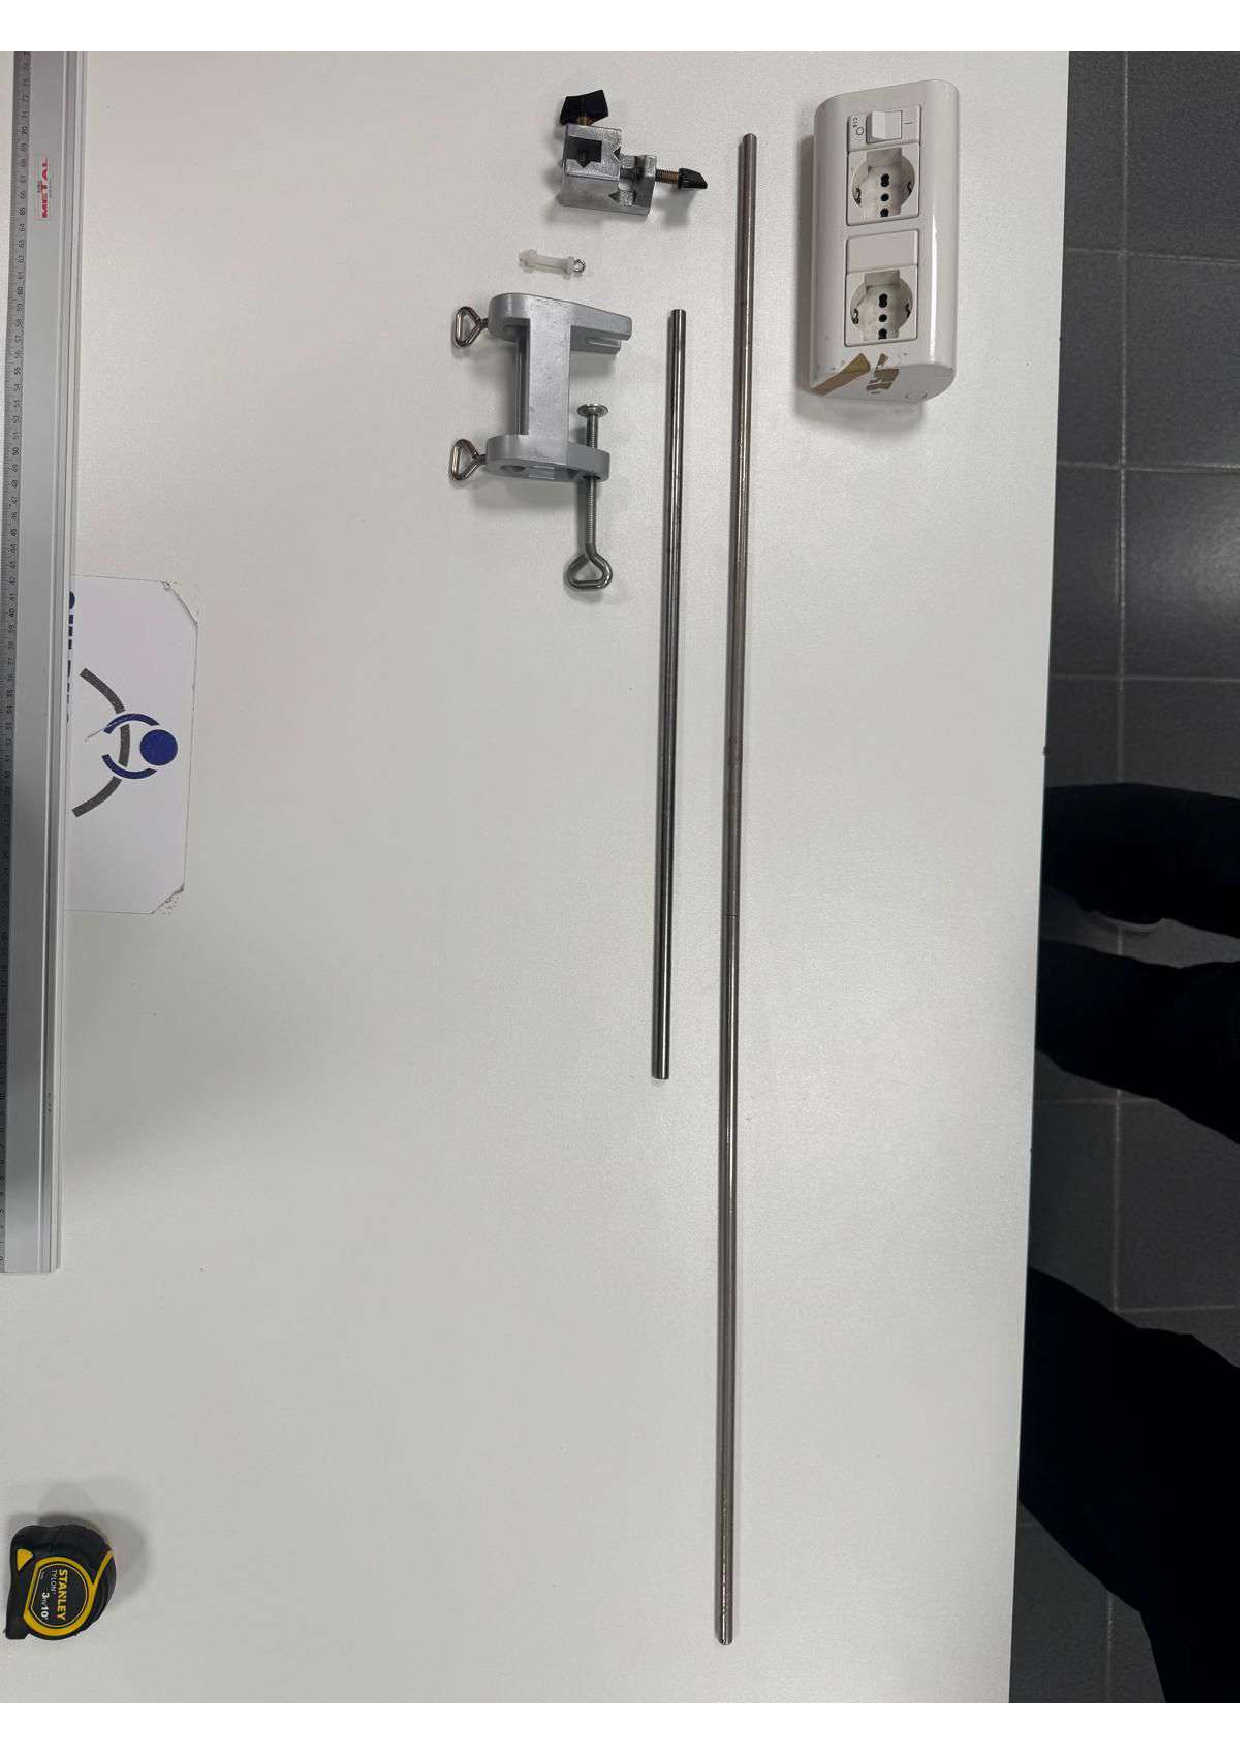
\includegraphics[width=0.35\textwidth]{pendolo.pdf}
  \caption{Componenti utilizzati per assemblare il pendolo}
\end{figure}

Il filo è stato fissato all'assa di supporto in modo da formare una "V". Questo, allo scopo di vincolare il moto del pesetto in un solo piano.
Per effettuare le misurazioni di massa, tempo e lunghezza ci siamo serviti della seguente strumentazione:
\begin{itemize}
    \item Bilancia digitale,
    \item Cronometro digitale,
    \item Metro analogico.
\end{itemize}

\begin{figure}[H]
  \centering
  \subfloat[Cronometro digitale]{%
    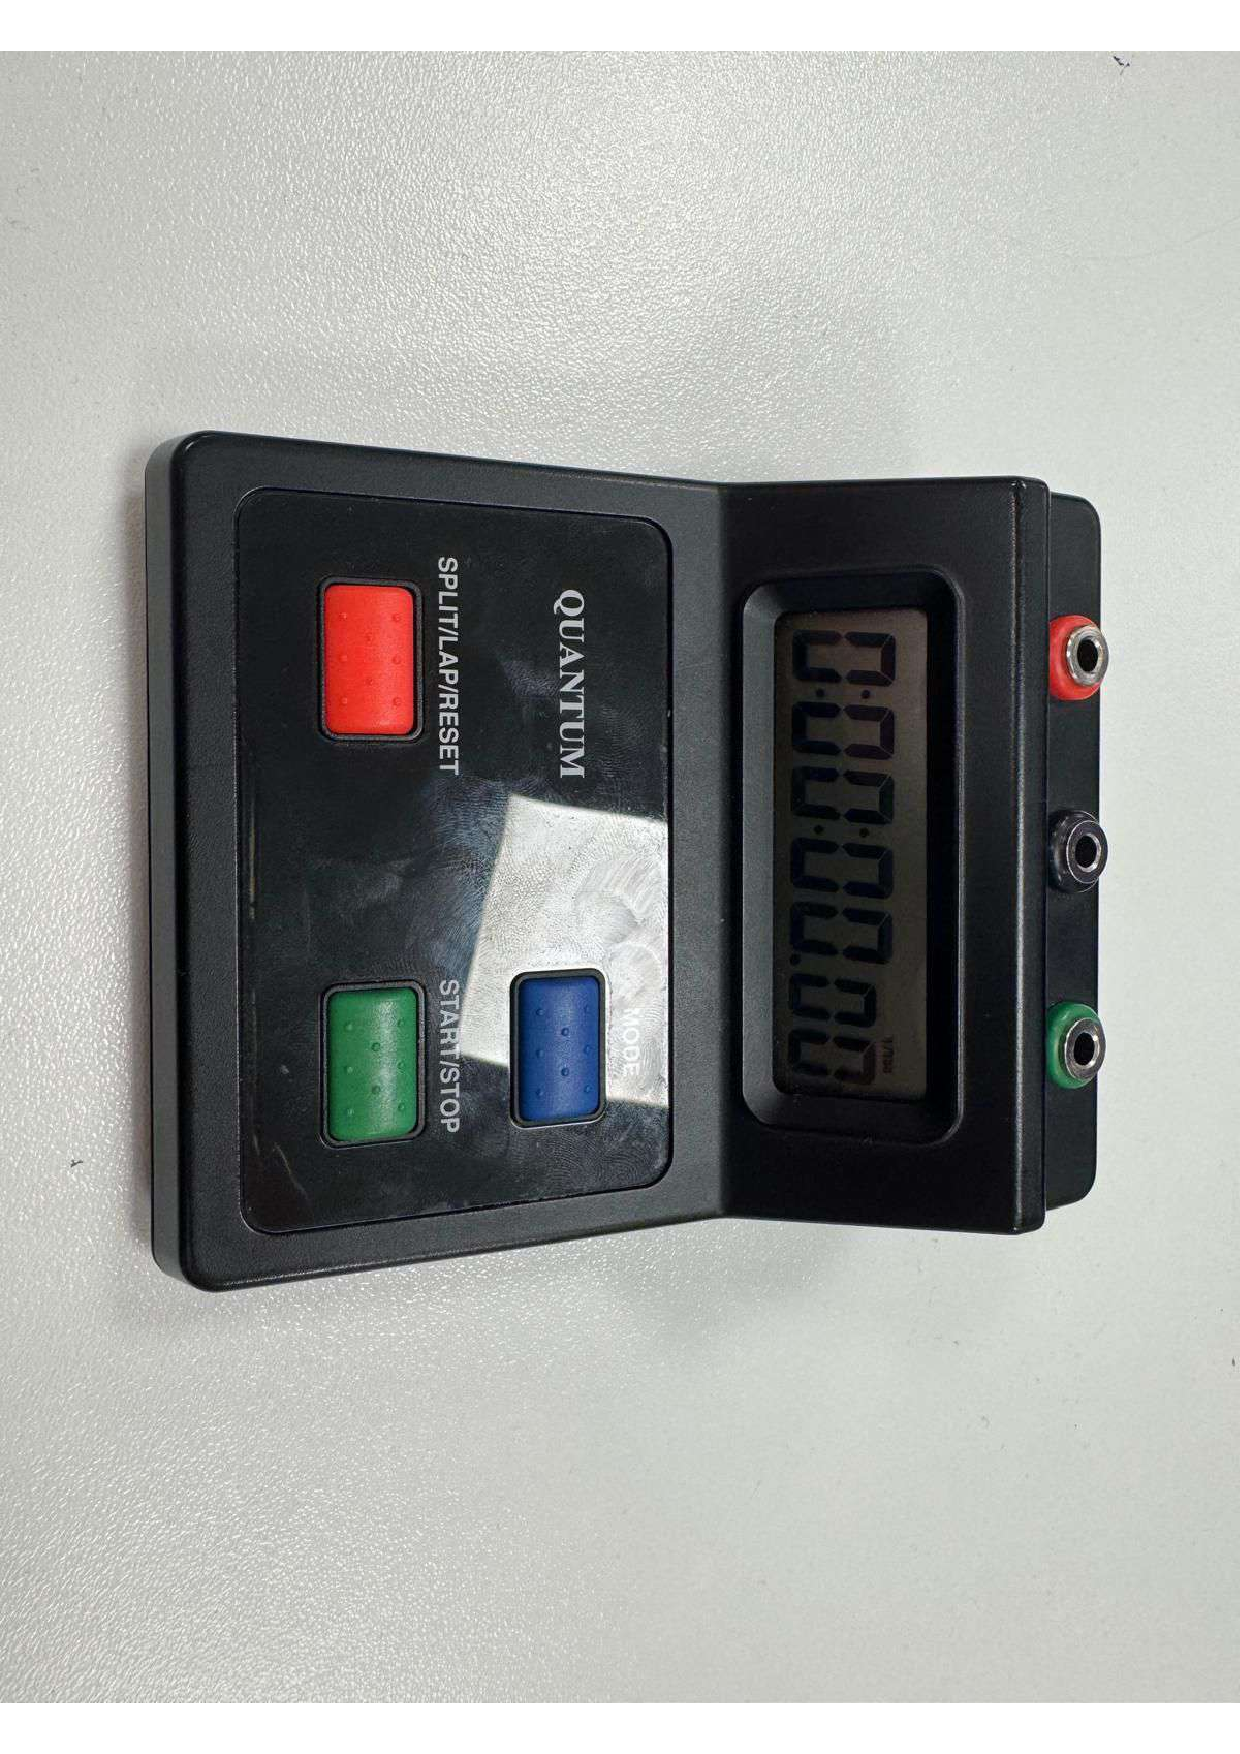
\includegraphics[width=0.45\textwidth]{cronometro.pdf}
  }
  \hspace{0.5cm} % Spazio tra le due immagini
  \subfloat[Metro analogico]{%
    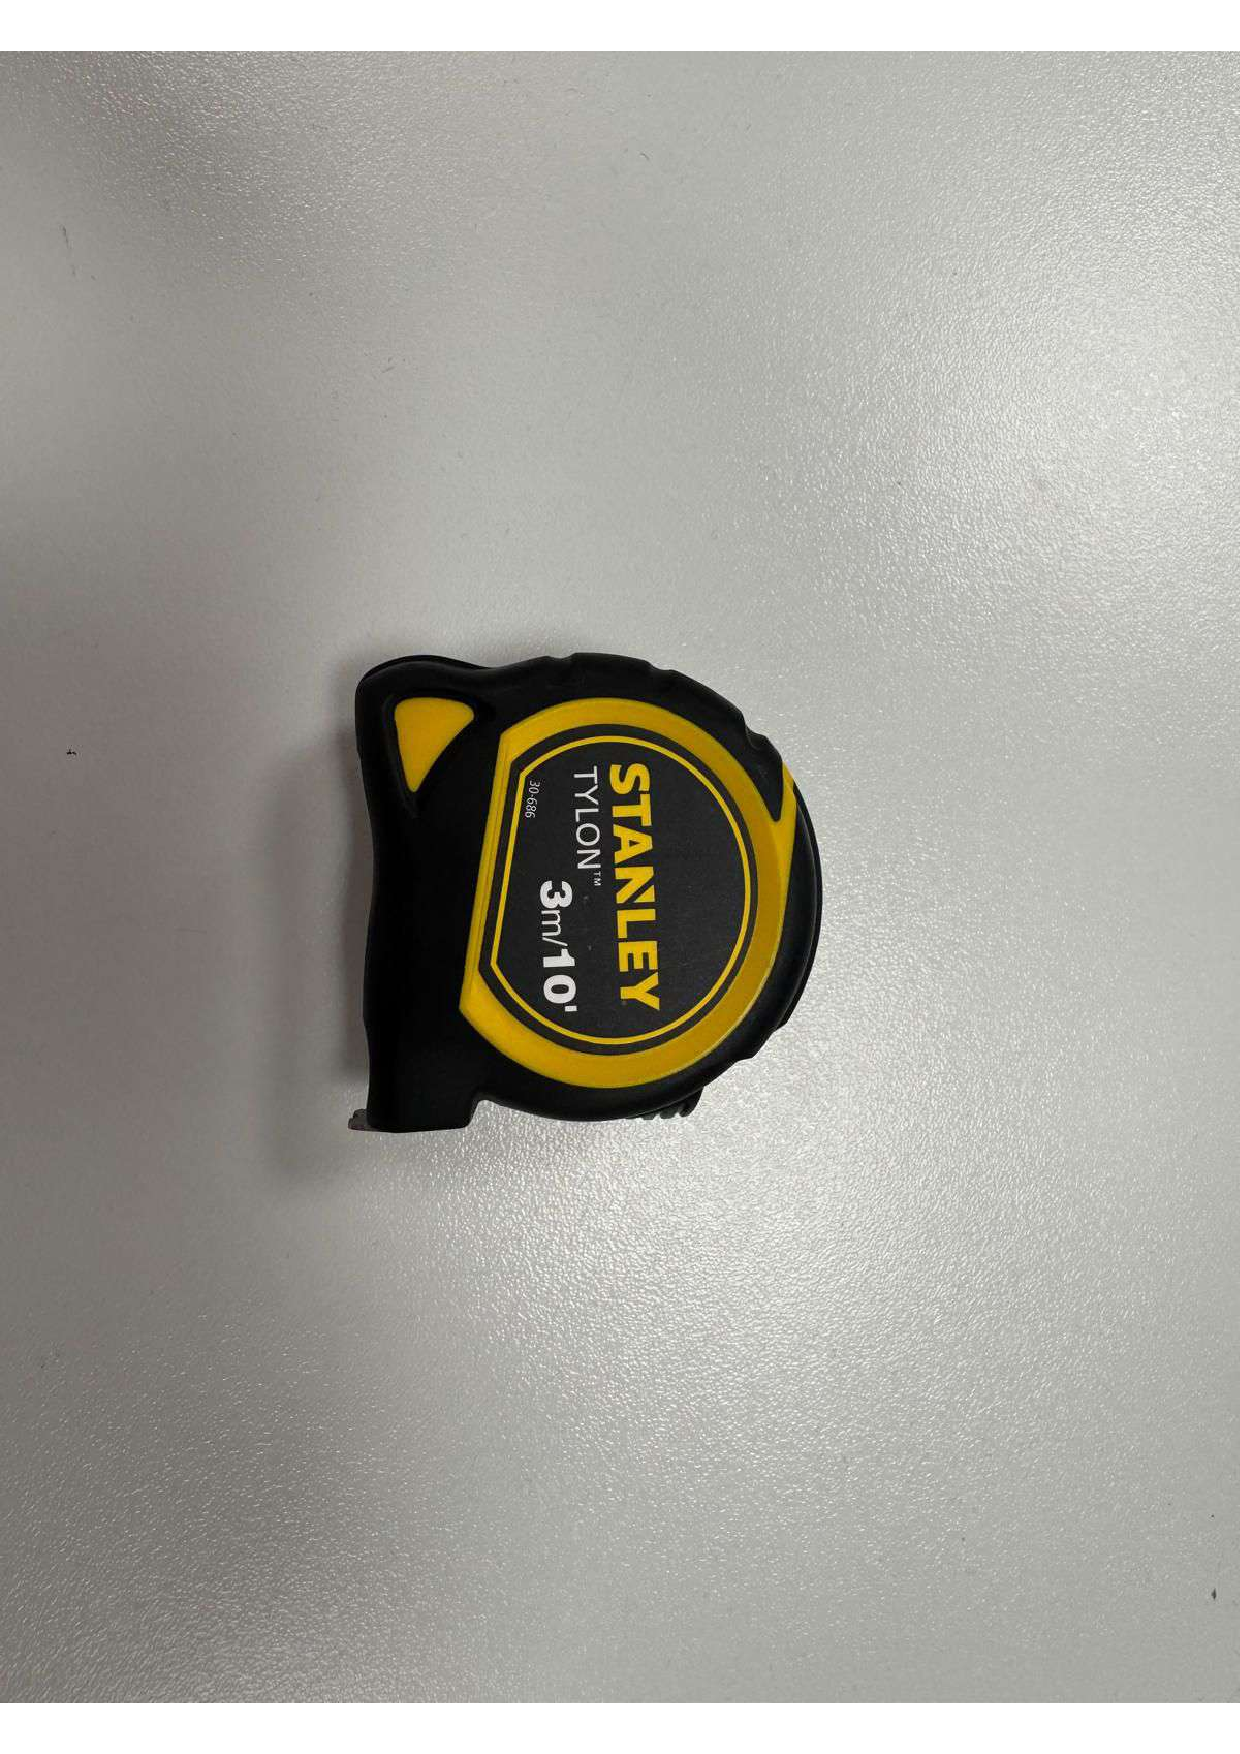
\includegraphics[width=0.45\textwidth]{metro.pdf}
  }
  \label{fig:due_immagini}
\end{figure}

\section{Descrizione e analisi dei dati sperimentali}

\subsection{Determinazione del regime di piccole oscillazioni }
Nella prima parte abbiamo messo in relazione il periodo d'oscillazione del pendolo con la sua ampiezza, cercando di individuare l'intervallo di piccole oscillazioni. L'ampiezza è stata misurata indirettamente, dalla relazione:
\begin{equation}
    \alpha=\arcsin(\frac{L}{I})
\end{equation}
dove $I$ e $L$ sono rispettivamente l'ipotenusa e il cateto maggiore del triangolo rettangolo che ha per base $L$ e per ipotenusa $I$. L'angolo $\alpha$ è quello intercettato dall'ipotenusa e dall'altezza. Il periodo di oscillazione è stato misurato direttamente, utilizzando il cronometro digitale. Per ogni ampiezza, la misurazione del periodo è stata ripetuta per cinque volte. L'errore assoluto sul periodo è stato valutato con la semidispersione. Per valutare l'incertezza sull'ampiezza si ricorre invece al metodo dei differenziali. Indicato con $\vec{x_0} = (L_0 , I_0)$ il vettore delle misure ottenute per le grandezze $L$ ed $I$ rispettivamente, si ottiene: 


\begin{align*}
    \Delta \alpha &= \left| \frac{\partial \alpha}{\partial L} \right|_{\vec{x} = \vec{x_0}} \Delta L + \left| \frac{\partial \alpha}{\partial I} \right|_{\vec{x} = \vec{x_0}} \Delta I = \\
    &= \left| \frac{1}{\sqrt{1 - (\frac{L}{I})^2}} \frac{1}{I}  \right|_{\vec{x} = \vec{x_0}} \Delta L + \left| \frac{1}{\sqrt{1 - (\frac{L}{I})^2}} \frac{-L}{I^2}  \right|_{\vec{x} = \vec{x_0}} \Delta I
\end{align*}

Per l'ampiezza è stata tenuta in considerazione la propagazione dell'errore dalle misurazioni dirette sulle lunghezze.

\begin{table}[H]
\centering
\begin{tabular}{|c|c|}
\hline
\textbf{Ampiezza ($rad$)} & \textbf{Periodo ($s$)} \\
\hline
$1.0972\pm 0.0015$ & $2.42\pm 0.05$ \\ 
$0.9732\pm 0.0014$ & $2.35\pm 0.02$ \\
$0.8799\pm 0.0012$ & $2.35\pm 0.03$ \\
$0.7723\pm 0.0012$ & $2.33\pm 0.02$ \\
$0.5560\pm 0.0011$ & $2.30\pm 0.05$ \\  
$0.3161\pm 0.0009$ & $2.26\pm 0.02$ \\
$0.1687\pm 0.0008$ & $2.27\pm 0.05$ \\
\hline
\end{tabular}
\caption{}
\label{tab:}
\end{table}

\begin{figure}[H]
  \centering
  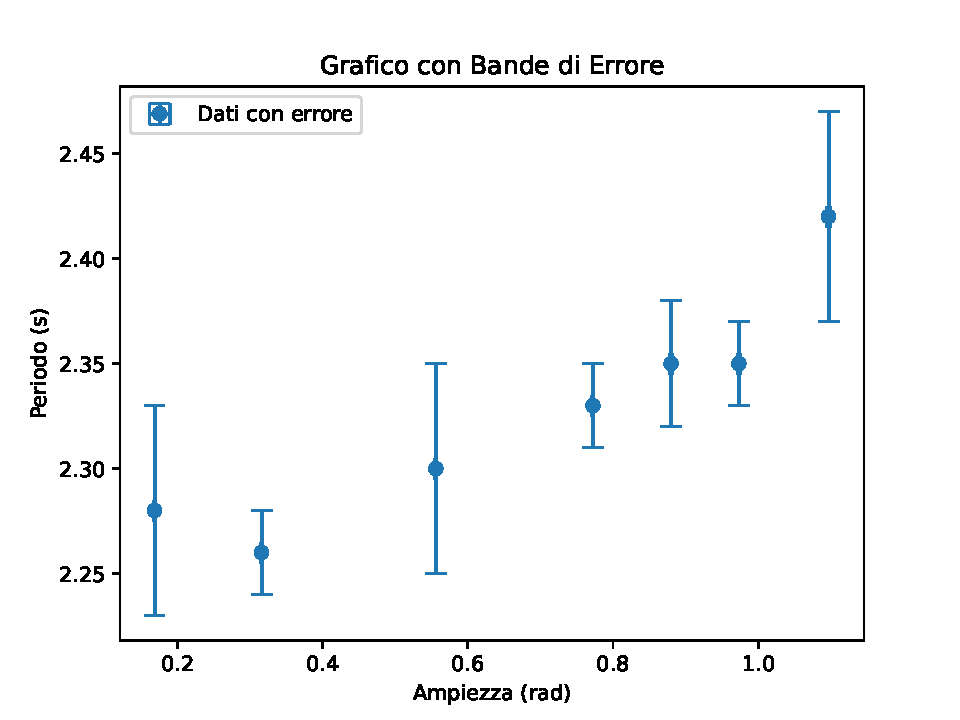
\includegraphics[width=1\textwidth]{grafico1p1.pdf}
  \caption{Il grafico rappresenta il periodo in funzione dell'ampiezza.}
\end{figure}

Notiamo che la discrepanza tra i periodi $(2.26\pm 0.02) s$ e $(2.27\pm 0.05) s$ è minore della somma delle due incertezze assolute per cui assumiamo che all'ampiezza $(0.3161\pm 0.0011) \ srad$ ci troviamo già nell'intervallo di piccole oscillazioni. Abbiamo continuato l'esperimento fissando questa ampiezza.
\\ \\
Sono state misurate diverse lunghezze del pendolo; per ognuna di queste abbiamo ricavato il periodo.

\begin{table}[H]
\centering
\begin{tabular}{|c|c|}
\hline
\textbf{Altezza ($cm$)} & \textbf{Periodo ($s$)} \\
\hline
$136.25\pm 0.05$ & $2.32\pm 0.01$ \\
$128.50\pm 0.05$ & $2.17\pm 0.01$ \\
$119.50\pm 0.05$ & $2.16\pm 0.01$ \\
$109.00\pm 0.05$ & $2.10\pm 0.01$ \\
$82.50\pm 0.05$ & $1.80\pm 0.01$ \\
$66.10\pm 0.05$ & $1.64\pm 0.01$ \\
$52.20\pm 0.05$ & $1.44\pm 0.01$ \\
$36.50\pm 1.24$ & $1.24\pm 0.01$ \\
\hline
\end{tabular}
\caption{}
\label{tab:}
\end{table}

Notiamo che al decrescere della lunghezza del pendolo, decresce il periodo d'oscillazione in accordo con la Legge (1).
Acquisiti questi dati, abbiamo costruito i seguenti grafici.

\begin{figure}[H]
  \centering
  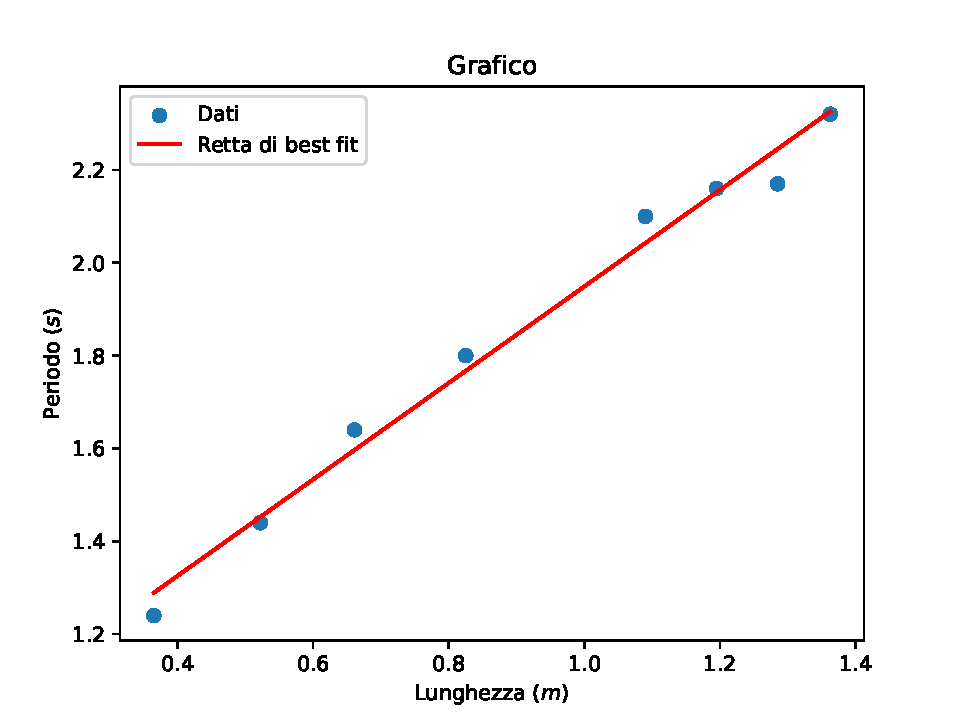
\includegraphics[width=1\textwidth]{grafico1p2.pdf}
  \caption{Il grafico rappresenta il periodo in funzione della lunghezza del pendolo.}
\end{figure}

\begin{figure}[H]
  \centering
  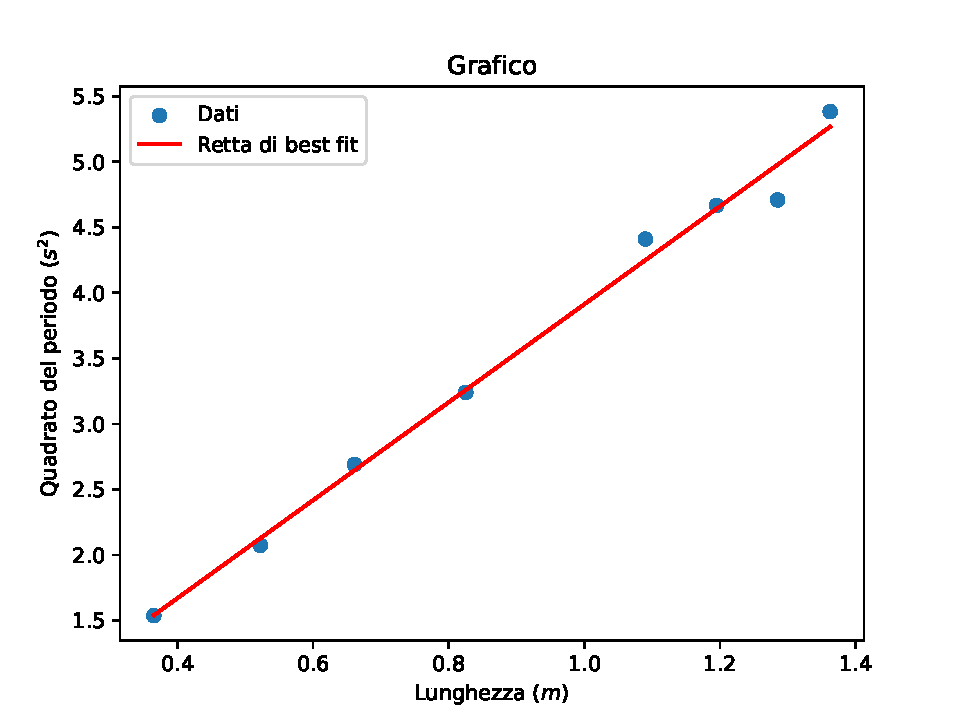
\includegraphics[width=1\textwidth]{grafico2p2.pdf}
  \caption{Il grafico rappresenta il quadrato del periodo in funzione della lunghezza del pendolo.\\ 
  Coefficiente angolare (b): $3.73643\pm 0.42422$ \\
  Intercetta (a): $0.17641\pm 0.41476$}
\end{figure}

\begin{figure}[H]
  \centering
  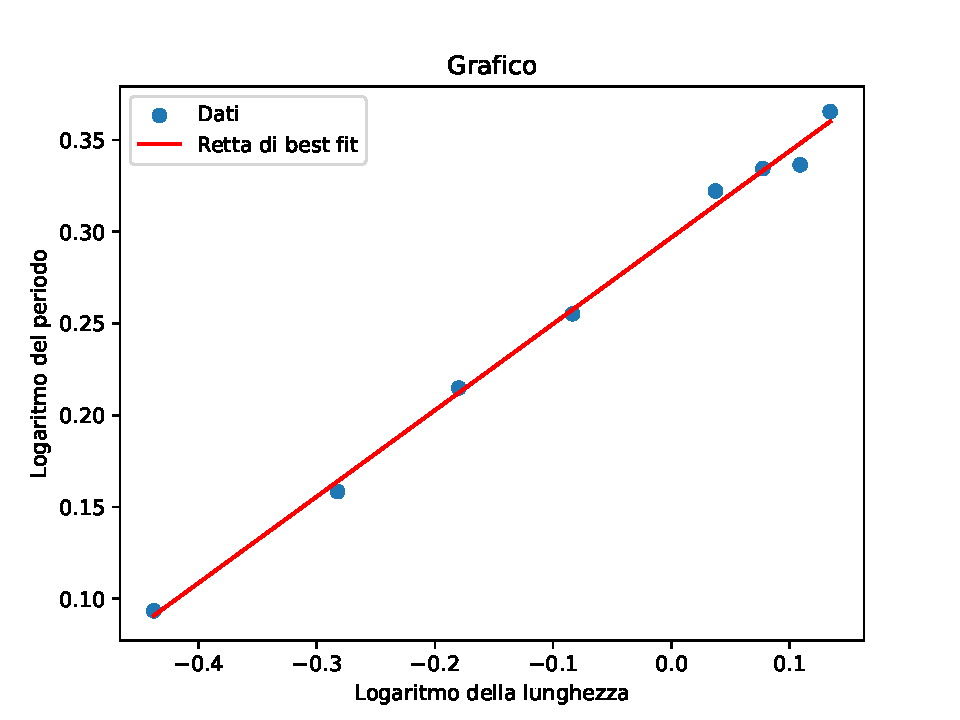
\includegraphics[width=1\textwidth]{grafico3p2.pdf}
  \caption{Il grafico rappresenta il logaritmo del periodo in funzione del logaritmo della lunghezza del pendolo. \\
  Coefficiente angolare (b): $0.47071\pm 0.03724$ \\
  Intercetta (a): $0.29686\pm 0.00777$}
\end{figure}

\begin{figure}[H]
  \centering
  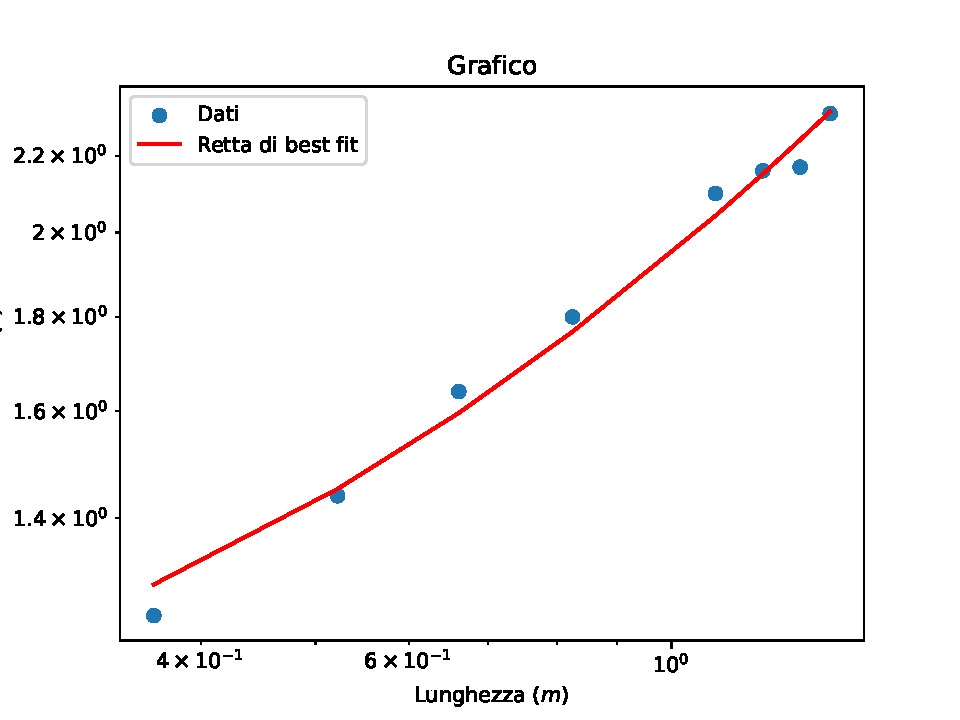
\includegraphics[width=1\textwidth]{grafico4p2.pdf}
  \caption{Il grafico rappresenta il periodo in funzione della lunghezza del pendolo in scala doppia logaritmica. Essendo in scala doppia logaritmica, la retta di best fit appare come una curva.}
\end{figure}
La stima del coefficiente angolare e dell'intercetta delle rette di best fit è stata effettuata utilizzando il metodo dei minimi quadrati.
Siano $b$ il coefficiente angolare e $a$ l'intercetta della retta:
\begin{equation}
    b=\frac{\displaystyle\sum_{i=1}^{N}[(x_i-\overline{x})(y_i-\overline{y})]}{\displaystyle\sum_{i=1}^{N}(x_i-\overline{x})^2}
\end{equation}
\begin{equation}
    a=\overline{y}-b\overline{x}
\end{equation}
Con $\overline{x}=\frac{\displaystyle\sum_{i=1}^{N}x_i}{N}$ e $\overline{y}=\frac{\displaystyle\sum_{i=1}^{N}y_i}{N}$
mentre le incertezze:
\begin{equation}
    \Delta b=3\sigma_b
\end{equation}
\begin{equation}
    \Delta a=3\sigma_a
\end{equation}
Con $$\sigma_b=\sigma_y\sqrt{\frac{N}{\Delta}}$$
$$\sigma_y=\sqrt{\frac{\displaystyle\sum_{i=1}^{N}(y_i-bx_i-a)^2}{N-2}}$$
$$\sigma_a=\sigma_y\sqrt{\frac{\displaystyle\sum_{i=1}^{N}x_i^2}{\Delta}}$$
$$\Delta=N\displaystyle\sum_{i=1}^{N}(x_i-\overline{x})^2$$


\section{Conclusioni}
Facendo riferimento alla Legge (5) e al coefficiente angolare della retta di regressione in Figura (4) possiamo calcolare il valore assoluto di $g$ e la sua incertezza assoluta $\Delta g$:
\begin{equation}
    g=4\pi^2b^{-1}
\end{equation}
\begin{equation}
    \Delta g = \frac{\Delta b}{b}g
\end{equation}
Sostituendo i valori ottenuti, si ottiene la seguente stima per $g$:
\begin{equation}
    \hat{g} = (10.56\pm 1.20)\frac{m}{s^2}
\end{equation}
Facendo riferimento alla Legge (6) e al termine noto della retta di regressione in Figura (5) si ottiene invece:
\begin{equation}
    g=(\frac{2\pi}{10^a})^2
\end{equation}
\begin{equation}
    \Delta g=\frac{\Delta a}{a}g
\end{equation}
E per $g$ la seguente stima:
\begin{equation}
    \hat{g}=(10.05\pm 0.26)\frac{m}{s^2}
\end{equation}
Sia la (14) che la (17) sono compatibili con il valore di riferimento
\begin{equation}
    g=9.81\frac{m}{s^2}
\end{equation}

poichè le loro incertezze assolute sono maggiori della loro discrepanza con la (18).

\end{document}